\documentclass[12pt,letterpaper]{article}
\usepackage[utf8]{inputenc}
\usepackage{tikz}
\usepackage{tkz-berge}
\usetikzlibrary {positioning}
\tikzset{LabelStyle/.style= {fill=white}}
\usepackage{amsfonts}
\usepackage{float}
\usepackage{mathrsfs}

\begin{document}
\begin{figure}[H]
    \centering
    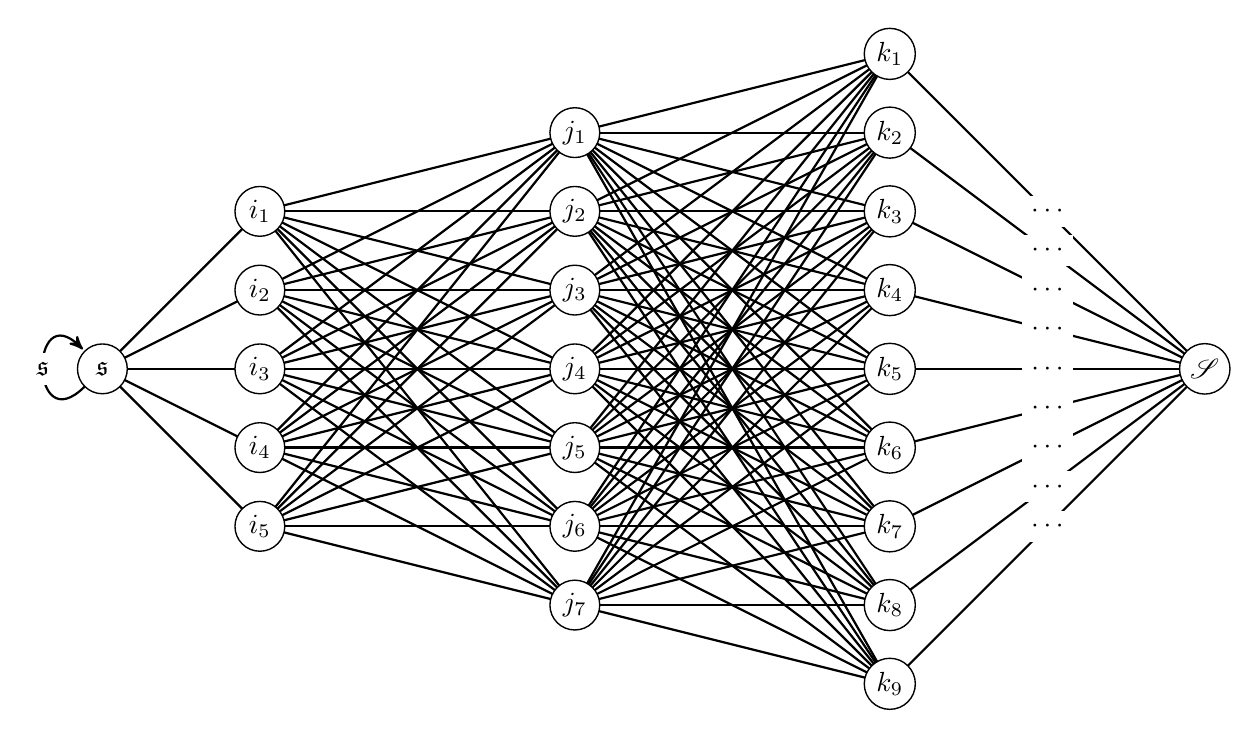
\begin{tikzpicture}
\SetVertexMath
\Vertex[x=0, y=0,L=\mathfrak{s}]{s}
\Loop[dist=1cm,label={$\mathfrak{s}$}](s)
\Vertex[x=14, y=0,L=\mathscr{S}]{S}

\Vertex[x=2, y=2, L=i_1]{l15}
\Vertex[x=2, y=1, L=i_2]{l14}
\Vertex[x=2, y=0, L=i_3]{l13}
\Vertex[x=2, y=-1, L=i_4]{l12}
\Vertex[x=2, y=-2, L=i_5]{l11}

\Edges(s, l11)
\Edges(s, l12)
\Edges(s, l13)
\Edges(s, l14)
\Edges(s, l15)

\Vertex[x=6, y=3, L=j_1]{l21}
\Vertex[x=6, y=2, L=j_2]{l22}
\Vertex[x=6, y=1, L=j_3]{l23}
\Vertex[x=6, y=0, L=j_4]{l24}
\Vertex[x=6, y=-1, L=j_5]{l25}
\Vertex[x=6, y=-2, L=j_6]{l26}
\Vertex[x=6, y=-3, L=j_7]{l27}

\Edges(l11, l21)
\Edges(l11, l22)
\Edges(l11, l23)
\Edges(l11, l24)
\Edges(l11, l25)
\Edges(l11, l26)
\Edges(l11, l27)

\Edges(l12, l21)
\Edges(l12, l22)
\Edges(l12, l23)
\Edges(l12, l24)
\Edges(l12, l25)
\Edges(l12, l26)
\Edges(l12, l27)

\Edges(l13, l21)
\Edges(l13, l22)
\Edges(l13, l23)
\Edges(l13, l24)
\Edges(l13, l25)
\Edges(l13, l26)
\Edges(l13, l27)

\Edges(l14, l21)
\Edges(l14, l22)
\Edges(l14, l23)
\Edges(l14, l24)
\Edges(l14, l25)
\Edges(l14, l26)
\Edges(l14, l27)

\Edges(l15, l21)
\Edges(l15, l22)
\Edges(l15, l23)
\Edges(l15, l24)
\Edges(l15, l25)
\Edges(l15, l26)
\Edges(l15, l27)

\Vertex[x=10, y=4, L=k_1]{l31}
\Vertex[x=10, y=3, L=k_2]{l32}
\Vertex[x=10, y=2, L=k_3]{l33}
\Vertex[x=10, y=1, L=k_4]{l34}
\Vertex[x=10, y=0, L=k_5]{l35}
\Vertex[x=10, y=-1, L=k_6]{l36}
\Vertex[x=10, y=-2, L=k_7]{l37}
\Vertex[x=10, y=-3, L=k_8]{l38}
\Vertex[x=10, y=-4, L=k_9]{l39}

\Edges(l21, l31)
\Edges(l21, l32)
\Edges(l21, l33)
\Edges(l21, l34)
\Edges(l21, l35)
\Edges(l21, l36)
\Edges(l21, l37)
\Edges(l21, l38)
\Edges(l21, l39)

\Edges(l22, l31)
\Edges(l22, l32)
\Edges(l22, l33)
\Edges(l22, l34)
\Edges(l22, l35)
\Edges(l22, l36)
\Edges(l22, l37)
\Edges(l22, l38)
\Edges(l22, l39)

\Edges(l23, l31)
\Edges(l23, l32)
\Edges(l23, l33)
\Edges(l23, l34)
\Edges(l23, l35)
\Edges(l23, l36)
\Edges(l23, l37)
\Edges(l23, l38)
\Edges(l23, l39)

\Edges(l24, l31)
\Edges(l24, l32)
\Edges(l24, l33)
\Edges(l24, l34)
\Edges(l24, l35)
\Edges(l24, l36)
\Edges(l24, l37)
\Edges(l24, l38)
\Edges(l24, l39)

\Edges(l25, l31)
\Edges(l25, l32)
\Edges(l25, l33)
\Edges(l25, l34)
\Edges(l25, l35)
\Edges(l25, l36)
\Edges(l25, l37)
\Edges(l25, l38)
\Edges(l25, l39)

\Edges(l26, l31)
\Edges(l26, l32)
\Edges(l26, l33)
\Edges(l26, l34)
\Edges(l26, l35)
\Edges(l26, l36)
\Edges(l26, l37)
\Edges(l26, l38)
\Edges(l26, l39)

\Edges(l27, l31)
\Edges(l27, l32)
\Edges(l27, l33)
\Edges(l27, l34)
\Edges(l27, l35)
\Edges(l27, l36)
\Edges(l27, l37)
\Edges(l27, l38)
\Edges(l27, l39)

\Edges[label={$\cdots$}](l31, S)
\Edges[label={$\cdots$}](l32, S)
\Edges[label={$\cdots$}](l33, S)
\Edges[label={$\cdots$}](l34, S)
\Edges[label={$\cdots$}](l35, S)
\Edges[label={$\cdots$}](l36, S)
\Edges[label={$\cdots$}](l37, S)
\Edges[label={$\cdots$}](l38, S)
\Edges[label={$\cdots$}](l39, S)
\end{tikzpicture}
    \caption{Graph of paths from the signifier \(\mathfrak{s}\) to the signified \(\mathscr{S}\)}\label{fig:graph}
\end{figure}
\end{document}